\section{Inference Scheme and Likelihood Function}\label{sec:inference}

In this Section, we describe the inference scheme and likelihood function by which our cosmological parameter constraints are derived from our emulator, the eBOSS flux power spectrum \cite{2019JCAP...07..017C} and the mean IGM temperature.
The overall inference scheme is:
\begin{enumerate}
    \item Use the emulator to predict the flux power spectrum and IGM mean temperature for a set of input parameters (see Table~\ref{tab:emulatorparams}).
    \item Calculate a likelihood comparing these predictions to their observational counterparts from eBOSS \cite{2019JCAP...07..017C} and Ref.~\cite{2021MNRAS.506.4389G}.
    \item Use Cobaya \cite{2021JCAP...05..057T, 2019ascl.soft10019T} to run MCMC chains and compute posterior parameter constraints.
\end{enumerate}
Section~\ref{sec:fpsdata} discusses the flux power spectrum data, while Section~\ref{sec:t0data} discusses the IGM temperature data.
We derive our covariance matrix in Section~\ref{sec:theoryerror}.
Details of the likelihood calculation used in the MCMC sampling are given in Section~\ref{sec:likelihood}.
We validate our pipeline on simulated data in Section~\ref{sec:simdat}.

% ------------------------------------------------------------------------------------
% ------------------------------------------------------------------------------------

\subsection{Flux Power Spectrum Data}
\label{sec:fpsdata}
% percent error for four surveys (calculated from their available data):
%                z_min     z_max     k_min      k_max      overall
% chabanier:     6%(2.2) 18%(4.6)    6%(0.001)  14%(0.02)     7% (4-18% over z, 5-14% over k)
% day:          15%(2)   14%(4.2)   15%(0.003)   14%(0.1)     11%
% karacayli:     7%(2)   27%(4.6)   12%(0.005)   9%(0.1)      9% (5-27% over z, 7-13% over k)
% irsic:        12%(3)   15%(4.2)   10%(0.003)  16%(0.06)     10%

We use the observed \lya forest flux power spectrum from \cite{2019JCAP...07..017C}, which is based on the Baryon Oscillation Spectroscopic Survey (BOSS) and extended-BOSS (eBOSS) quasar samples \cite{2013AJ....145...10D, 2016AJ....151...44D}.
In \cite{2019JCAP...07..017C}, the BOSS/eBOSS quasar samples are refined to remove spectra that have not been visually inspected, and to remove spectra with broad absorption lines.
Sky lines and damped \lya absorbers (DLAs) are masked.
Our simulations include a realistic population of DLAs, which are masked in the same way.

The sample of \lya forests from the set of remaining quasar spectra is then further refined based on cuts to the spectral resolution, signal-to-noise ratio, number of masked pixels, and forest length, with a final sample of about $43,000$ spectra.
%Along with a windowing function to correct for the spectral resolution of the instrument, estimates for the noise and metal power (estimated using longer wavelength segments of the quasar spectra) are then subtracted to obtain the final \lya forest flux power spectrum.
The redshifts and scales covered by these observations set the redshift range and scales we use in our flux power spectrum emulator, namely $z=2.2-4.6$ (redshift bin size of $\Delta z = 0.2$), and $k\approx0.001-0.02$ s/km (over $35$ linearly spaced bins, $\Delta k = 5.42\times10^{-4}$ s/km).
Note, our emulator can easily be re-trained for the smaller scales probed by DESI.
The average uncertainty in the \lya forest flux power from Ref.~\cite{2019JCAP...07..017C} ranges from $\approx6\%$ at low redshifts or large scales, to $\approx16\%$ for high redshifts or small scales, and is often dominated by systematic uncertainty.

We apply correction terms to the \lya forest flux power spectrum predicted by our emulator to model DLAs and metal contamination.
We correct for DLAs using the template from Ref.~\cite{2018MNRAS.474.3032R}.
This allows us to account for differences in the DLA masking between our simulated pipeline and the observed pipeline.
An example would be DLAs, or Lyman limit systems (LLS), which are not detected in the observational pipeline due to low spectral signal-to-noise.
Note that our simulation includes a model that produces realistic populations of LLSs and DLAs, so the marginalised template allows for aspects in which the simulated model differs from the real Universe.
In \cite{2018MNRAS.474.3032R}, there are four parameters, with sub-DLAs separate from LLSs, and DLAs divided into two categories.
For each of the parameters, a redshift and scale dependent correction is applied, where a positive (negative) value for the parameter implies that our simulation has underestimated (overestimated) the number of absorbers in that category. 
We found that in practice our dataset was unable to measure separately all four of the column density bins.
We thus simplify our likelihood by using only two additional free parameters, one parameter covering sub-DLAs and LLS, $\alpha_{\mathrm{lls}}$, and one parameter covering DLAs, $\alpha_{\mathrm{dla}}$.
$\alpha_{\mathrm{lls}}$ covers column densities between $1.6\times10^{17} - 10^{20}$ cm$^{-2}$), and $\alpha_{\mathrm{dla}}$ covers $10^{21}-10^{22.5}$  cm$^{-2}$. 

We account for correlated Si~{\sc{iii}} absorption within the \lya~forest following Ref.~\cite{2006ApJS..163...80M}.
Our likelihood includes an additional nuisance parameter, $f_\mathrm{SiIII}$, which measures the amplitude of the metal contamination. 

% -------------------------------------------------------------------------------------------------

\subsection{IGM Mean Temperature Data}\label{sec:t0data}

We use the mean IGM temperatures from Ref.~\cite{2021MNRAS.506.4389G}, derived from simulation modeling of high resolution quasar spectra from the KODIAQ survey \cite{2017AJ....154..114O}.
Ultimately the dataset is a relatively small, visually inspected set of high resolution quasar spectra.
Importantly, these spectra are independent of the eBOSS quasar sample, justifying our choice of separate likelihood functions.
We include IGM mean temperature data for $z=2.2-3.8$, for consistency with the available \lya forest flux power data.
The average uncertainty for this data set is $\approx10\%$, whereas our mean temperature emulator has an average uncertainty of $\sim 1\%$.
Ref.~\cite{2021MNRAS.506.4389G} provides mean temperatures derived from four different statistics: the \lya forest flux power spectrum, curvature, wavelet decomposition, and Doppler width distribution.
We use the \lya forest flux power spectrum derived temperatures in the main body of this work, but show results using these other data sets in Appendix~\ref{sec:t0-only}.

%In \cite{2021MNRAS.506.4389G}, their co-added quasar spectra are manually checked, and the sample is refined to remove spectra that do not contain \lya forest, do contain DLAs or sub-DLAs, have large gaps in the spectra, or do not meet a signal-to-noise ratio cut.
% A cut is also made to remove regions of the spectra that may lie near to a quasar proximity zone.
%Metal lines are removed by fitting Voigt profiles to the spectra and removing features with Doppler widths $b \leq 8$ km s$^{-1}$, which are assumed to be metal lines.
To derive temperatures from the observed quasar spectra, Ref.~\cite{2021MNRAS.506.4389G} calculated several summary statistics and compared them to those derived from spectra drawn from simulations.
The simulations they used were similar in resolution to our HF suite (gas mass resolution of $\sim10^5$ M$_{\odot}$), though much smaller in volume ($10$ Mpc/h box side length).
Because these observed mean temperatures are themselves derived using a suite of simulations, it would be optimal to remove the middle step in future work, i.e. calculate mean temperatures using the observed small-scale 1D flux power spectrum and our own set of simulations.

% ---------------------------------------------------------------------------

\subsection{Covariance Matrix}
\label{sec:theoryerror}

\begin{figure}
    \centering
    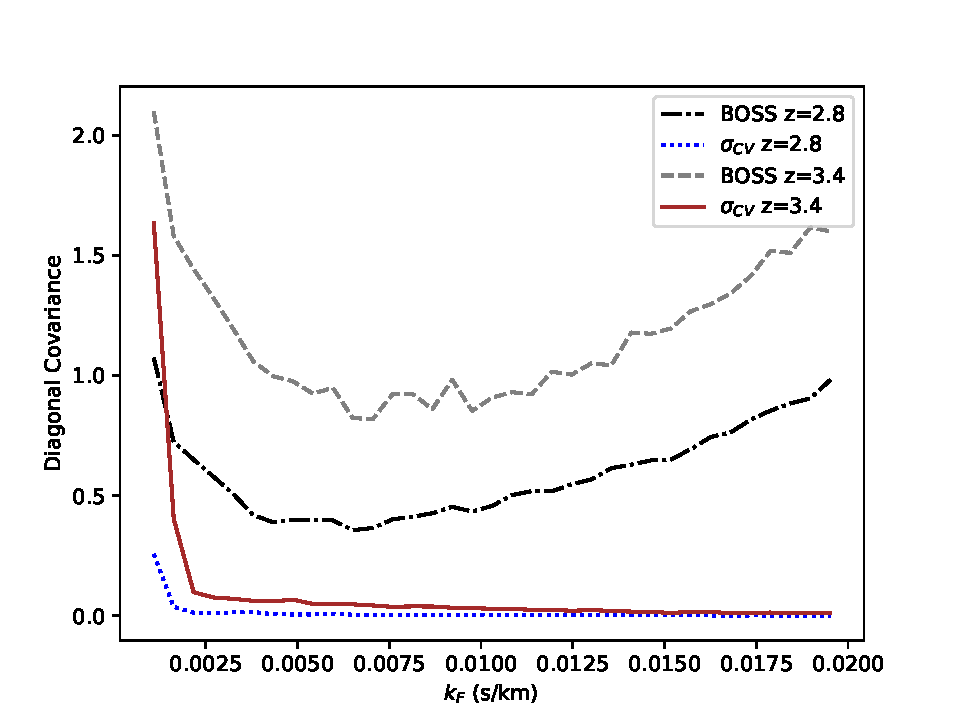
\includegraphics[width=\textwidth]{figures/errors_loo.pdf}
    \caption{\label{fig:covariance_loo}
    Diagonal elements of the covariance matrix as a function of scale and for selected redshift bins.
    Shown are the square root of the diagonal elements of the eBOSS covariance matrix and the diagonal cosmic variance error estimated from leave-one-out errors, $\boldsymbol{\sigma}_{CV}$.}
\end{figure}

In this Section, we derive the covariance matrix, $\boldsymbol{K}$, that is used for our inference.
We decompose $\boldsymbol{K}$ as:
\begin{equation}
    \boldsymbol{K} = \boldsymbol{K}_\mathrm{BOSS} + \boldsymbol{\sigma}_{GP}(\boldsymbol{p}) \cdot \boldsymbol{\sigma}_{GP}^T (\boldsymbol{p}) + \boldsymbol{\sigma}_{CV} \cdot \boldsymbol{\sigma}_{CV}^T \,.
    \label{eq:covariance}
\end{equation}
Here, $\boldsymbol{K}_\mathrm{BOSS}$ is the covariance matrix from the eBOSS pipeline \cite{2019JCAP...07..017C}, and is the largest term in the covariance matrix on most scales.
We also add two extra terms which model theoretical error in our model.
$\boldsymbol{\sigma}_{GP}(\boldsymbol{p})$ is the parameter dependent estimate of the interpolation error from the Gaussian process.
We found that in some cases when a parameter was poorly constrained this could unphysically drive the chain towards the edge of parameter space where the interpolation error was large.
We thus choose to omit it from the overall covariance matrix.
Appendix~\ref{sec:loovsgperr} shows that its addition has a small effect on our final results.

The second theoretical error in our simulation suite (which dominates) is $\boldsymbol{\sigma}_{CV}$, which models residual sample variance from the finite box size, analogous to cosmic variance from the finite cosmological horizon\footnote{Ref.~\cite{2023ApJ...944..223P} reduced sample variance by interpolating the parameters of a higher order polynomial, rather than fitting the binned flux power spectrum directly.
Our emulator is much less affected by sample variance as our simulated volume is $8$ times larger.}.
We include an estimate of sample variance using the leave-one-out errors discussed in Ref.~\cite{2023simsuite}, a technique made possible by the inclusion of $h$ in our simulation suite.
The Hubble parameter does not directly affect the gravitational evolution in our simulations due to Gadget's use of Mpc/h units, and Ref.~\cite{2023simsuite} showed that the effect on the thermal history is small on the scales probed by eBOSS.
However, in our parameterization, $h$ also changes $\Omega_M$ \footnote{$\Omega_M h^2$ is a separate parameter and so kept fixed when varying $h$.} \maf{should this be $\Omega_M h^2$?} \spb{No, the point is that varying h for fixed OmegaMh2 also changes OmegaM} and so the conversion of wavenumbers from h/Mpc to s/km.
Individual Fourier modes thus move between bins depending on the value of $h$, mimicking the sample variance from different initial phases.
We thus approximate $\boldsymbol{\sigma}_{CV}$ with the averaged variance of the leave-one-out errors using the low fidelity simulations.
Leave-one-out errors are found by building a reduced emulator, which is trained on all but a single sample, then evaluating the prediction accuracy for that left-out sample using the reduced emulator.
This is then repeated, such that every sample takes a turn being left out (see Figure~2 of \cite{2023simsuite}):
\begin{equation}
    \boldsymbol{\sigma}^2_{CV}  = \frac{1}{N_{LF}}\Sigma_i \left(P_F^\mathrm{Predict}(k, z, p_i) - P_F^\mathrm{True}(k, z, p_i)\right)^2\,.
\end{equation}
Here the sum runs over all simulated low-fidelity parameter sets $p_i$ and $N_{LF}$ is the number of low-fidelity simulations. 

Figure~\ref{fig:covariance_loo} shows the magnitude of the $\boldsymbol{\sigma}_{CV}$ term compared to the eBOSS errors.
$\boldsymbol{\sigma}_{CV}$ is significant only on the largest scales, $k < 2.5 \times 10^{-3}$ s/km, as expected from an effect due to finite box size.
In addition, there is a significant redshift dependence: $\boldsymbol{\sigma}_{CV}$ is large compared to the eBOSS errors only for $2.8 < z < 3.4$.
For clarity, Figure~\ref{fig:covariance_loo} shows only $z=2.8$ and $z=3.4$. However, we have verified that $\boldsymbol{\sigma}_{CV}$ reduces for lower redshifts. For the redshift range $4.2 > z>3.4$, $\boldsymbol{\sigma}_{CV}$ remains approximately constant, but becomes less significant as the eBOSS statistical errors increase. \maf{not sure I totally follow this sentense in the context of the figure} \spb{Is that better?}.
These details reveal the physical source of this large-scale variance.
The relevant scale is close to the $20$ Mpc/h size of the Helium reionization bubbles, and the relevant redshift range is when our model performs helium reionization.
Helium reionization bubbles are placed randomly around rare large halos, which creates sample variance in a finite box.

\subsection{Likelihood}\label{sec:likelihood}

We use a log normal likelihood summed over all redshifts and, for the flux power, all scale bins:
\begin{equation}
    \mathrm{log}\mathcal{L} = -\frac{1}{2} \sum_{z=2.2}^{z=4.6} \left(\boldsymbol{P}_F^{\mathrm{diff}} \cdot \boldsymbol{K}^{-1} \cdot \boldsymbol{P}_F^{\mathrm{diff}} + \mathrm{det}(\boldsymbol{K})\right)
    \label{eq:likelihood}
\end{equation}
where $\boldsymbol{P}_F^{\mathrm{diff}} = \boldsymbol{P}_F^{\mathrm{sim}} - \boldsymbol{P}_F^{\mathrm{obs}}$ is the vector difference between the simulation prediction and the observation.
The covariance matrix, $\boldsymbol{K}$, is described in Equation~\ref{eq:covariance}. 

The likelihood for the IGM mean temperature is similar, but single valued per redshift.
We compute the \lya forest flux power and IGM mean temperature likelihoods separately.
Because the flux power spectrum has larger magnitude likelihoods (due to the extra dimension of information, $k$, and additional redshift bins), the mean temperature likelihood is scaled by a factor of $\sim 10$, to ensure both information sources contribute roughly equally to the posterior.

We make use of the Cobaya package \cite{2021JCAP...05..057T, 2019ascl.soft10019T, 2013PhRvD..87j3529L, 2002PhRvD..66j3511L} to run MCMC chains using this likelihood.
The MCMC sampler uses the Metropolis method discussed in \cite{2013PhRvD..87j3529L}, and uses a Gaussian + exponential proposal distribution that dynamically learns the proposal covariance.
Convergence is determined using the Gelman-Rubin statistic, $R$, also detailed in \cite{2013PhRvD..87j3529L}.
The chains presented here were all run until a convergence of $R-1 < 0.01$, with results plotted for those chains for samples at $R-1 < 1$.

\subsubsection{Priors}

We use the parameter limits shown in Table~\ref{tab:emulatorparams}.
As we showed in Ref.~\cite{2023simsuite}, the AGN feedback parameter $\epsilon_{AGN}$ has minimal effect on the \Lya forest 1D flux power spectrum.
Preliminary chains indicated that it is indeed poorly constrained by the data and has minimal correlations with other parameters.
We use a strong Gaussian prior with $\mu = 0.05$ and $\sigma = 0.005$, which dominates over data constraints, and will omit constraints on $\epsilon_{AGN}$ from our results.
We also place a weak Gaussian prior on the Hubble parameter, $h$, with $\mu = 0.70$ and $\sigma = 0.015$, as it is weakly constrained and this prior avoids the inference straying into areas near the edge of parameter volume where the emulation is less accurate.
For all other parameters we use uniform priors within the parameter limits.

\subsection{Inference Using Simulation Data}\label{sec:simdat}

In this section we test our inference framework with simulation outputs in place of the observational data, confirming that we recover the known input parameters.
We first used the flux power spectrum from one of the three high fidelity simulations, and confirmed that the maximum likelihood was indeed at the input parameter values for all parameters.
All input parameters were recovered to better than one sigma.

\begin{figure}
    \centering
    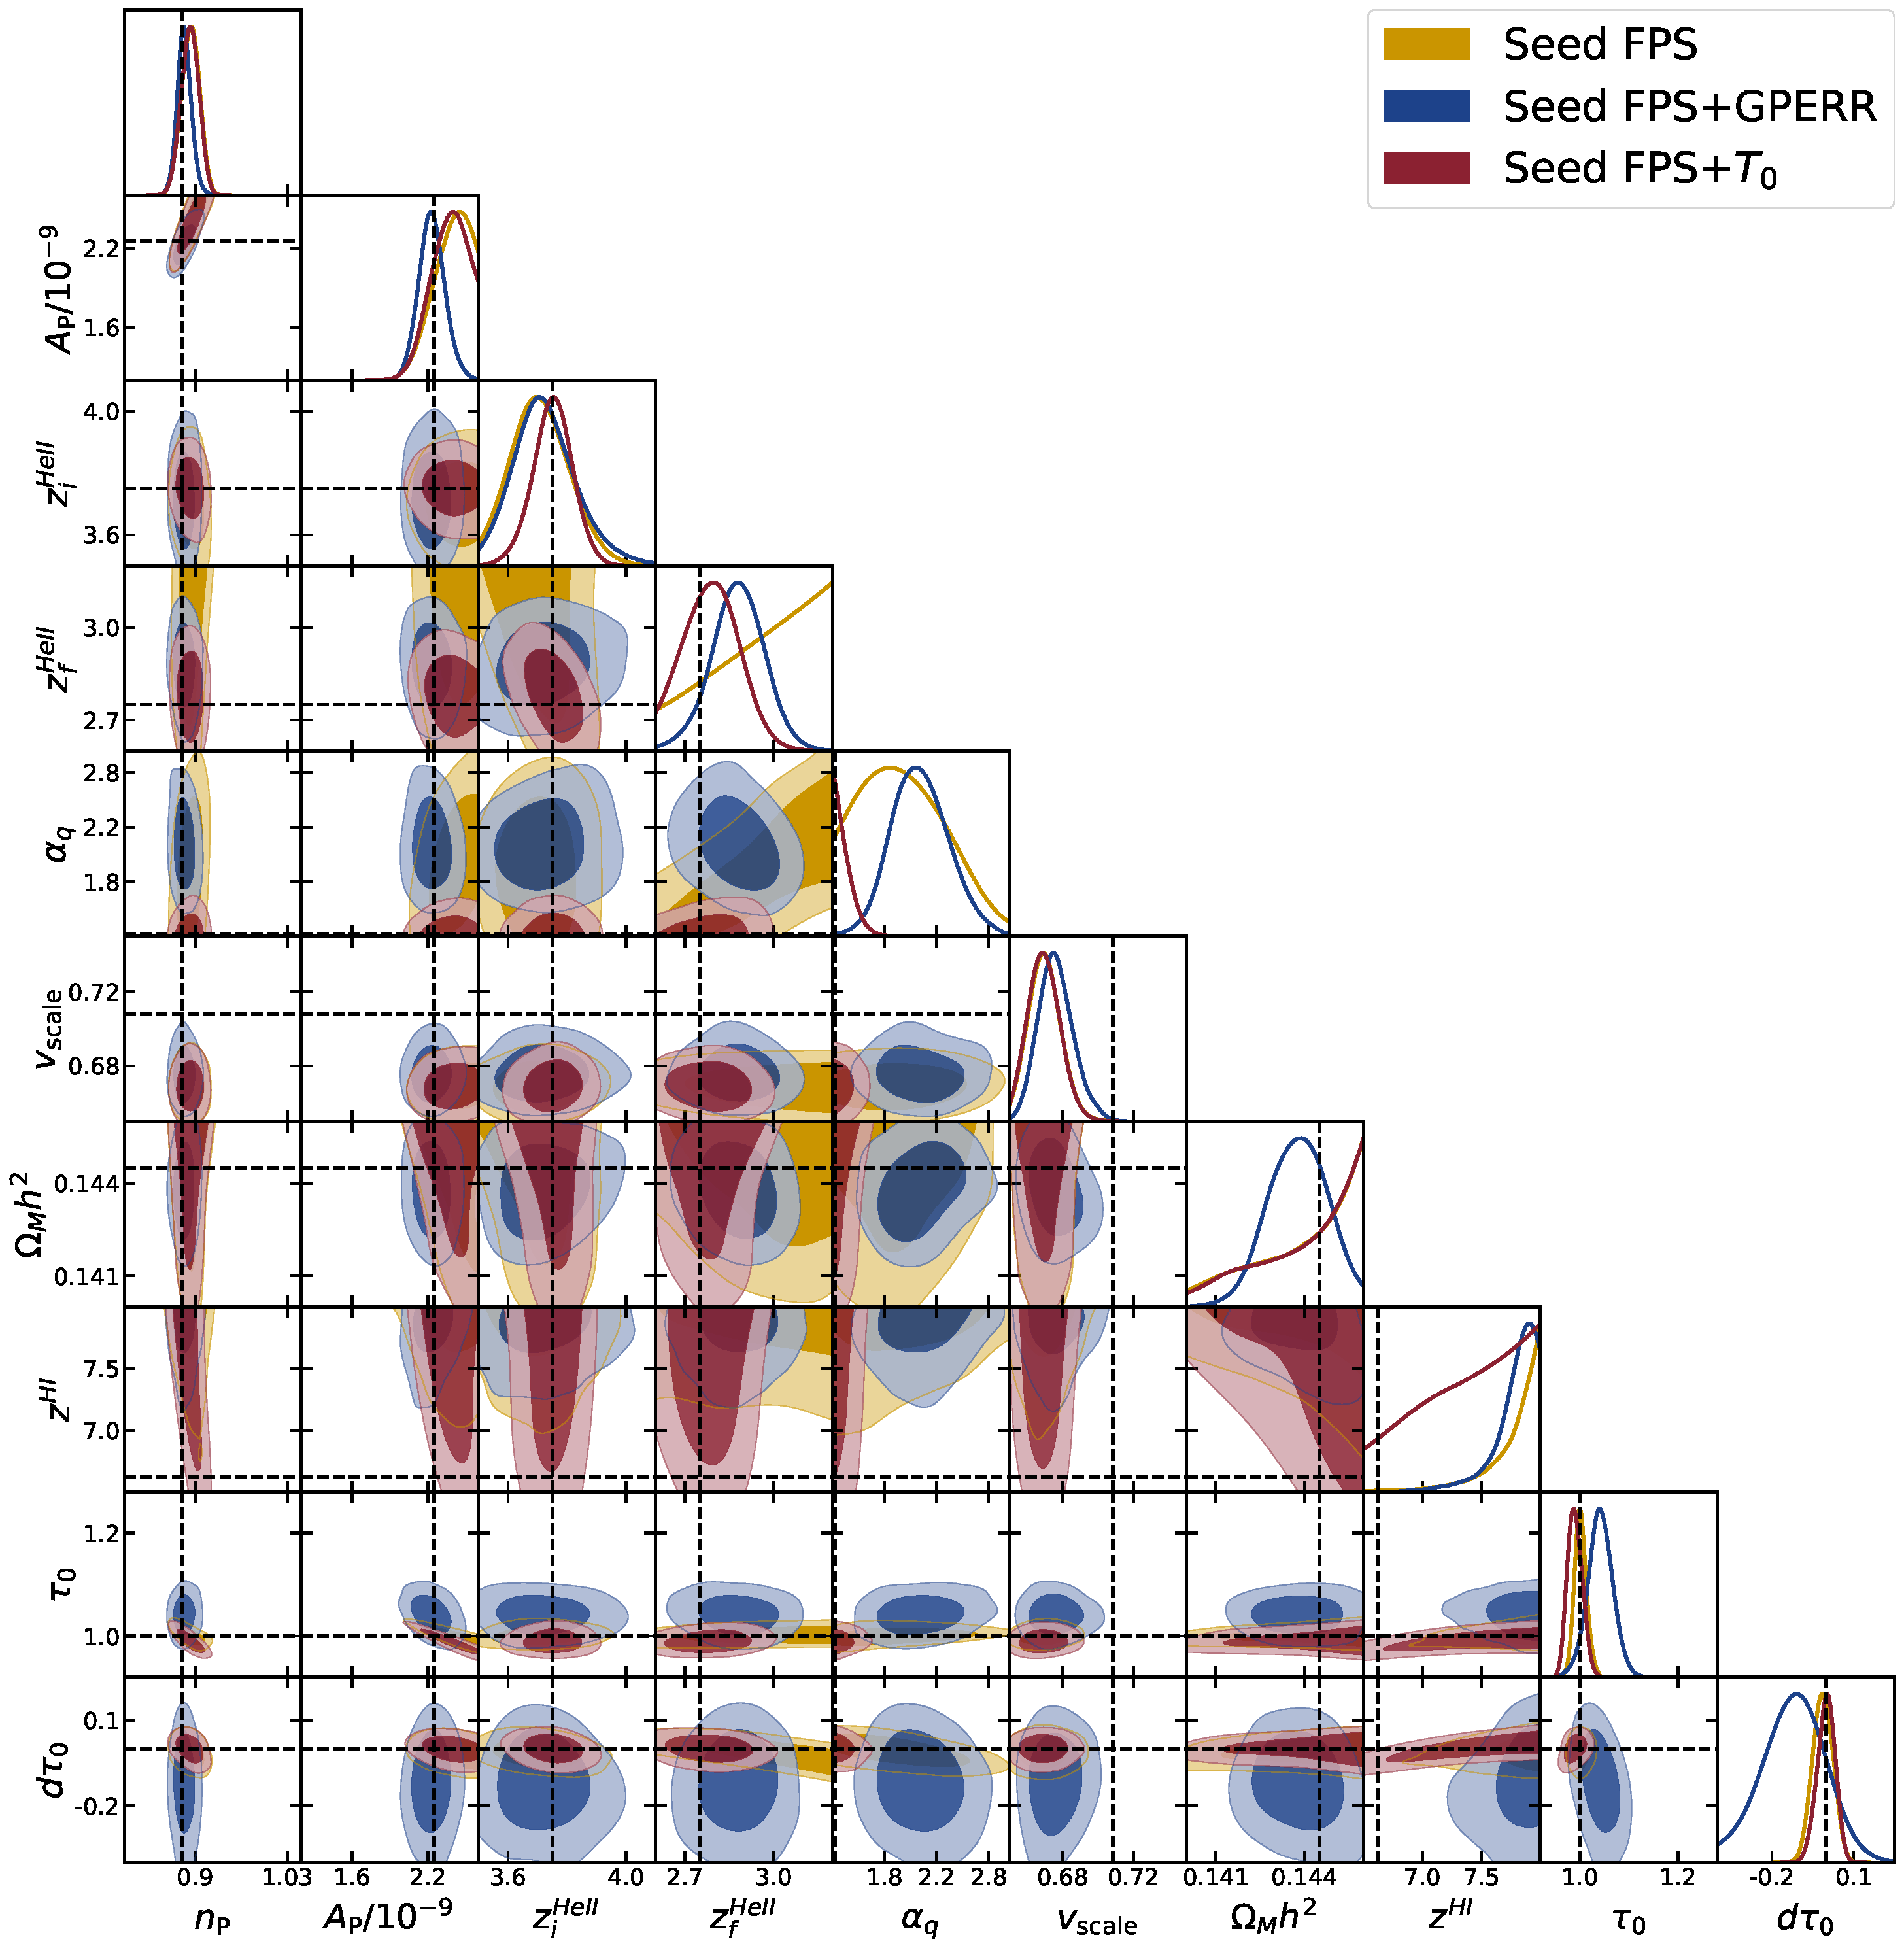
\includegraphics[width=\textwidth]{figures/simdat-seed.pdf}
    \caption{\label{fig:simdat_posteriors}
    \maf{if not too much trouble, maybe change the dashed line color -- blue might work} \spb{How's that? I went with black so that there weren't too many colours floating around.}
    Posteriors using mock data, a simulation output with a different initial seed to the main PRIYA suite.
    The true parameter values for the input are indicated by the red dashed lines.
    Three chains are used: `Seed FPS' uses the default error model, with the eBOSS covariance and leave-one-out errors.
    `Seed FPS + GPERR' adds the covariance from the Gaussian Process.
    `Seed FPS + $T_0$' uses the default error model but supplements the flux power spectrum data with information from the mean temperature.
    $v_{scale}$ is the Hubble parameter $h$, re-labelled for reasons explained in the text.}
\end{figure}

We next ran chains using data from a low-fidelity simulation with a different random seed from the main PRIYA suite.
For these runs only, we used an emulator built using the low fidelity suite.
This test was designed to quantify whether the finite box size of our simulations can affect our parameter constraints.
Figure~\ref{fig:simdat_posteriors} shows the results, with dashed red lines indicating the correct parameters.

We have performed three runs.
The first (Seed LOO) is our preferred error model, using the eBOSS covariance and a leave-one-out (LOO) error term.
The second adds an error term for the expected interpolation error from the Gaussian Process (Seed LOO + GP).
Both of these runs use only information from the eBOSS flux power spectrum and thus do not provide strong constraints on the parameters of helium reionization.
We therefore run another chain including constraints from the mean temperature.

In all three runs, the optical depth parameters, $\tau_0$ and $d\tau_0$, are tightly constrained around the true value in our pipeline, despite the effect of a different structure seed. The GPERR chain increases the uncertainty, especially on $d\tau_0$, but does not bias the measurement.
The best estimate comes from the flux power spectrum data alone (Seed FPS).
We also consistently recover the true values of the cosmological parameters $n_P$ and $A_P$, although $A_P$ is about $1-\sigma$ high for the chain which includes the mean temperature.
This is not unreasonable as we deliberately constructed our test data, with a different structure seed, to be different from the training data.
$\Omega_M h^2$ is poorly constrained in all chains, as expected given that our prior volume includes only a narrow range for $\Omega_M h^2$, motivated by Planck results.
All parts of the prior range are within the $1-\sigma$ posteriors.

The redshift of hydrogen reionization, $z_{HI}$, is estimated from the mean IGM temperature at $z > 3.6$ or from a large-scale increase in the flux power spectrum at $z > 4$ (see Ref.~\cite{2023simsuite}).
The second effect is due to a scale-dependent bias arising from placement of the reionization bubbles \cite{Montero:2019}.
Figure~\ref{fig:simdat_posteriors} indicates that this bias is sensitive to sample variance from the finite box, and so the hydrogen reionization redshift is not well measured by the flux power spectrum data alone.
The three parameters which govern Helium reionization, $z_i^{HeII}$, $z_f^{HeII}$ and $\alpha_q$, are well constrained by the mean temperature data.
The runs which do not include mean temperature data have a preference for a larger $\alpha_q$ than the input value.
As discussed above, the main effect of a different structure seed is through the placement of Helium reionization bubbles.
$\alpha_q$ is thus measured using a similar scale-dependent bias as $z_{HI}$, and so is slightly sensitive to the finite box size in the same way.
However, the mean IGM temperature is sensitive to $\alpha_q$ through the peak temperature during Helium reionization, and thus the chains including it correctly infer $\alpha_q$.

The chain including Gaussian Process errors sometimes produced incorrect parameter inferences, notably in $\alpha_q$.
It seems that GP errors create an implicit prior which sometimes shifts the results towards regions of higher interpolation accuracy.
The simulated data seems to exaggerate this effect, perhaps because of the exact choice of simulated parameters near the edge of the prior volume.
We show in Appendix~\ref{sec:loovsgperr} that the posteriors from eBOSS data are not significantly changed by including GP error.
Nevertheless, to be conservative our main results are reported with chains run omitting GP errors from the likelihood.

As discussed above, the Hubble parameter, $h$, does not affect the evolution of our simulations except through its effect on $\Omega_M$ (at fixed $\Omega_M h^2$) and thus the scaling between velocity (km/s) and comoving (Mpc/h) units.
Constraints on $h$ ($v_\mathrm{scale}$) are incorrect in the chains shown in Figure~\ref{fig:simdat_posteriors}, driven by sample variance in the finite box.
We confirmed that gradients of the likelihood with respect to $h$ are largest for the largest scales, particularly the first $4$ $k$-bins.
We computed the $\chi^2$ per degree of freedom, which was $\sim 0.9$ for $h = 0.65$ and $\chi^2 \sim 1$ for the true input value, indicating over-fitting to the noise created by different structure seeds.
We confirmed that fixing $h$ to the known true value results in very small changes to the other parameters and their confidence intervals.
There is thus zero cosmological information in our $h$ constraints.
In order to avoid unwarranted conclusions, we will henceforth relabel $h$ as $v_\mathrm{scale}$, emphasising that it merely controls the mapping between the native Fourier-space binning of the simulations and the observed velocity space of the spectra, and its inference is dominated by modelling error from sample variance.